\documentclass[a4paper,12pt]{article}

\usepackage[utf8]{inputenc}
\usepackage{lmodern}
\usepackage[margin=1cm]{geometry}
\usepackage{amsmath}
\usepackage{graphicx}
\usepackage{xcolor}
\usepackage{caption}
\usepackage{tikz}
\usetikzlibrary{arrows.meta,positioning,shapes.geometric,calc,fit}

\pagestyle{empty}

\begin{document}
\begin{figure}[p]
  \centering
  \makebox[\textwidth][c]{\resizebox{1.05\textwidth}{!}{%
  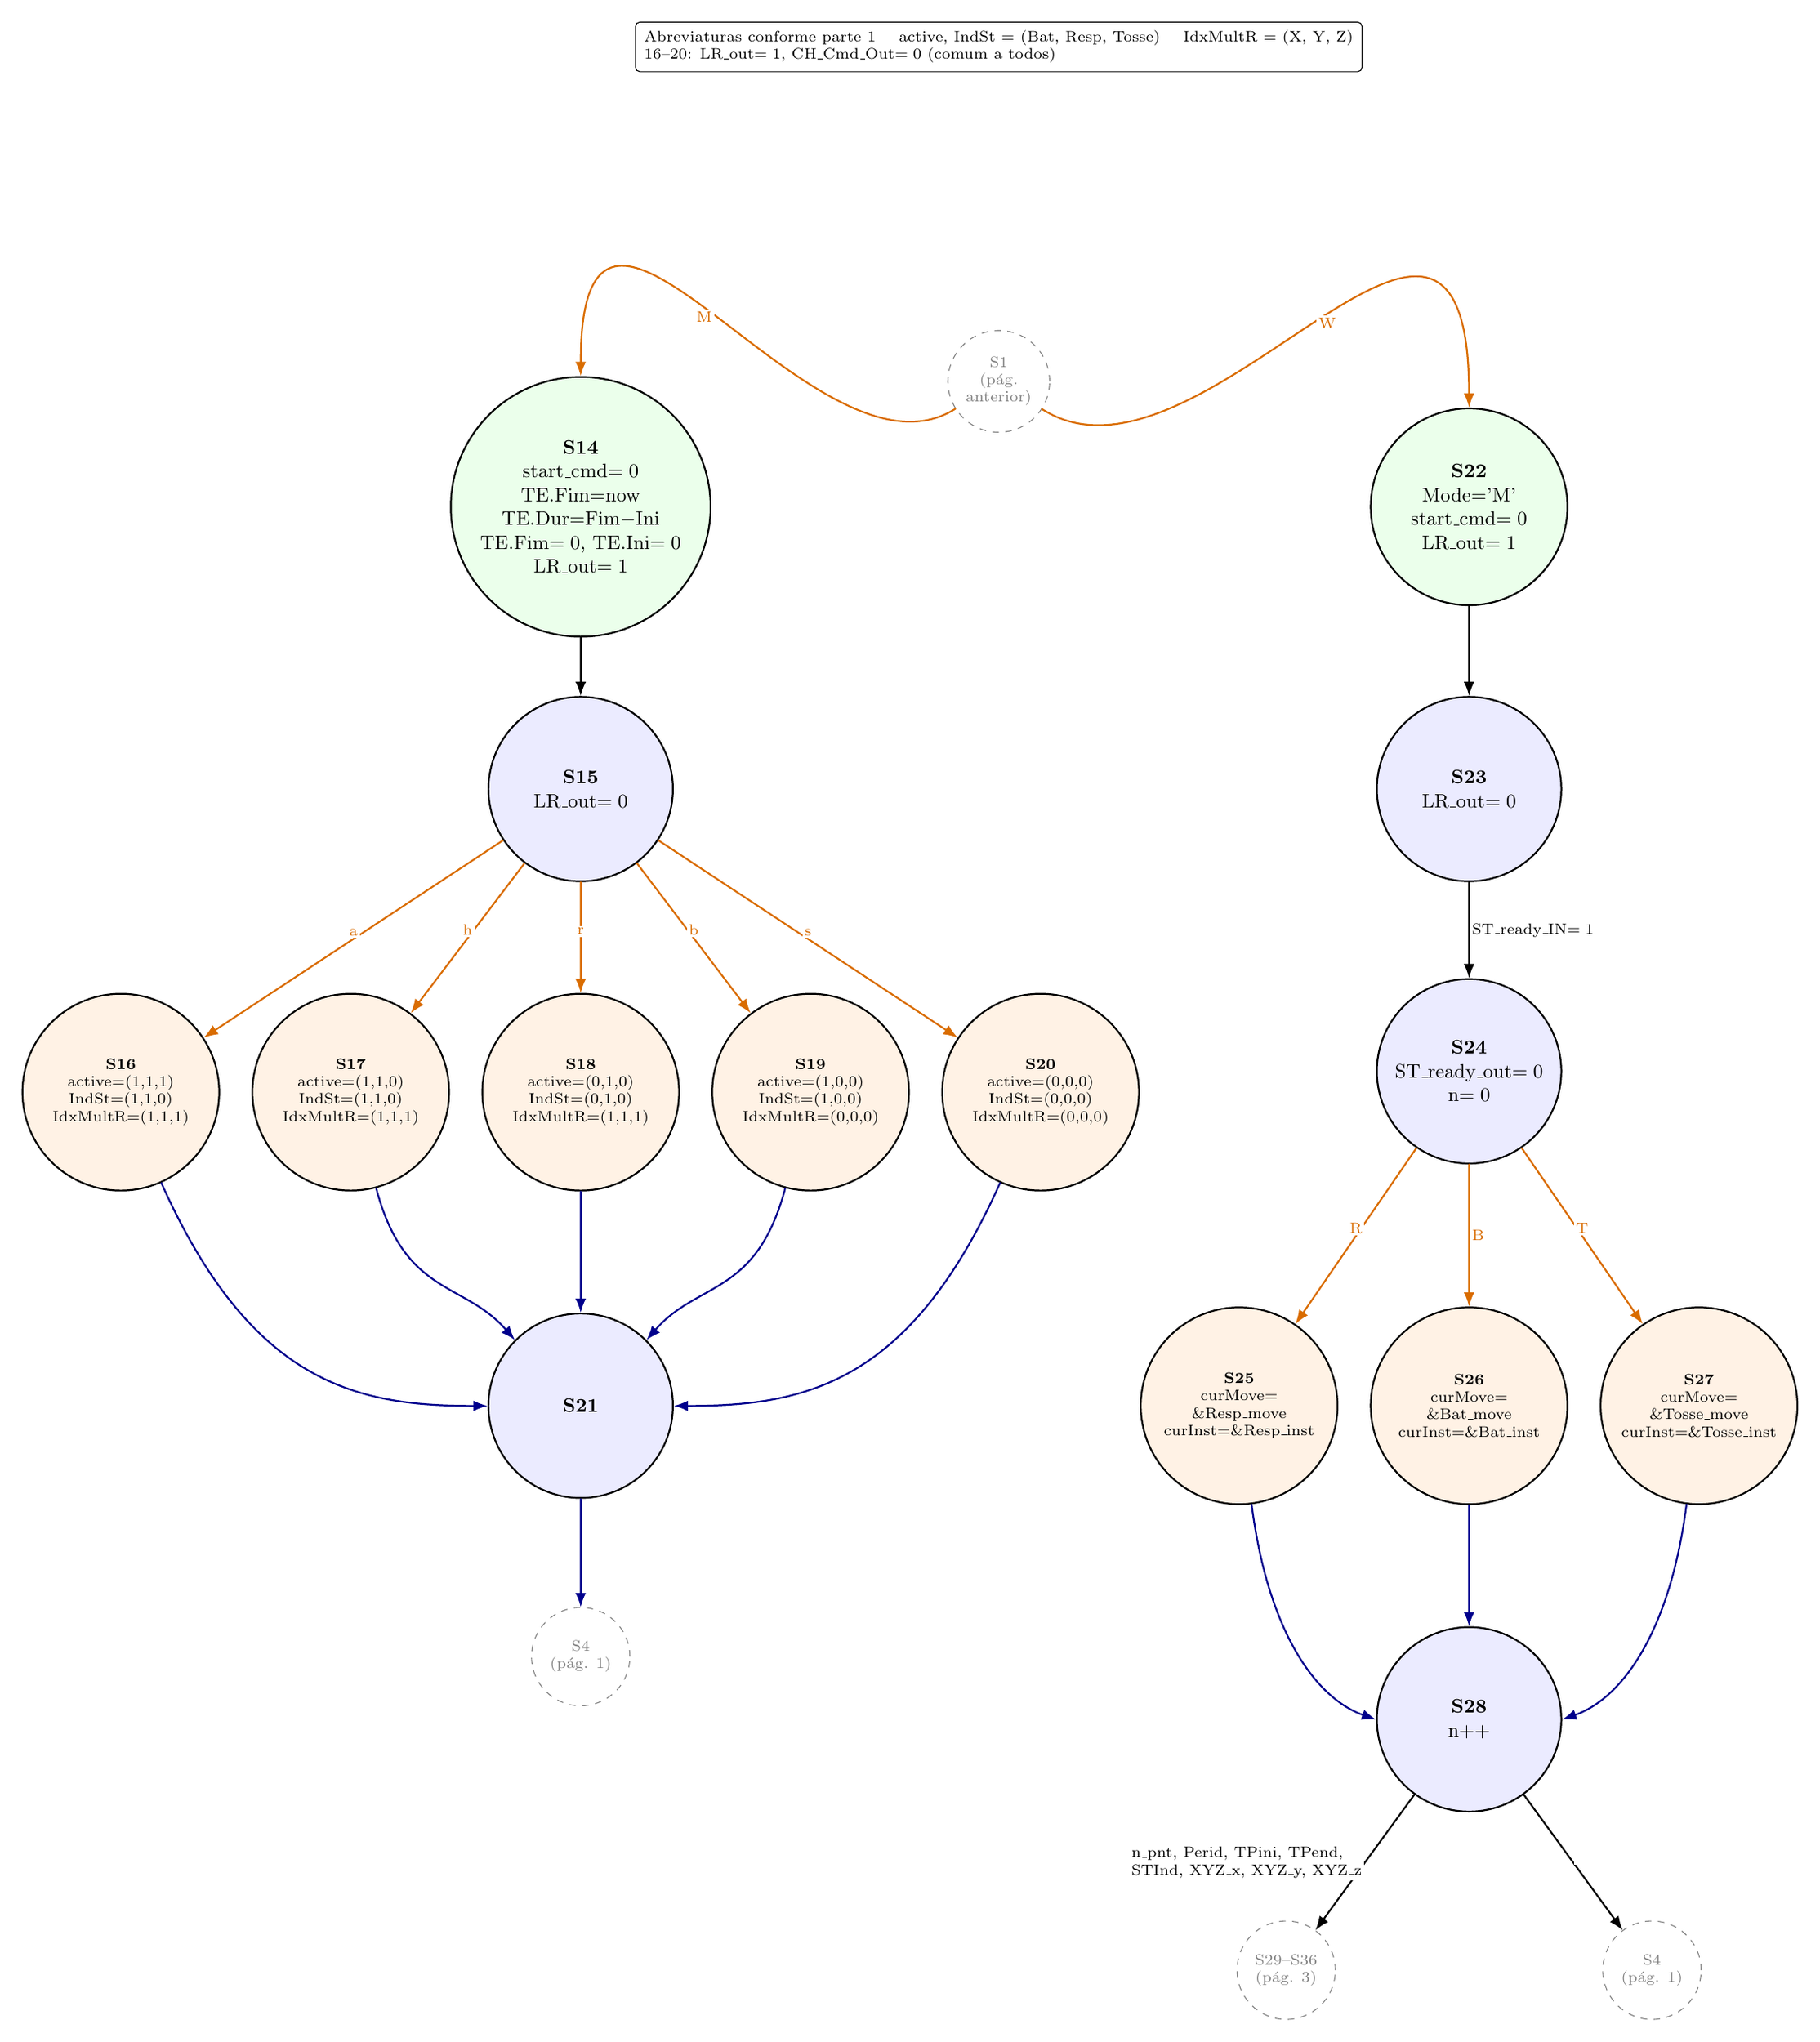
\begin{tikzpicture}[
    xscale=0.85, yscale=1.7,
    state/.style={draw, circle, align=center, minimum size=3.0cm, font=\small, thick},
    proxy/.style={draw, dashed, circle, align=center, minimum size=1.6cm, font=\scriptsize, gray},
    arrow/.style={-Latex, thick, line cap=round, line join=round},
    cmd/.style={-Latex, thick, orange!85!black, line cap=round, line join=round},
    ret/.style={-Latex, thick, blue!55!black, line cap=round, line join=round},
    lab/.style={font=\scriptsize, align=center, fill=white, inner sep=1pt},
    >=Stealth
  ]
    \node[draw, rounded corners=2pt, align=left, font=\scriptsize, fill=white, inner sep=4pt] at (3.0,4.4)
      {Abreviaturas conforme parte 1 \quad active, IndSt = (Bat, Resp, Tosse) \quad IdxMultR = (X, Y, Z)\\
       16--20: LR\_out$=1$, CH\_Cmd\_Out$=0$ (comum a todos)};

    \node[proxy] (p1a) at (3.0,1.2) {S1\\(pág.\\anterior)};

    \node[state, fill=green!8, minimum size=3.4cm] (c14) at (-5.0,0)     {\textbf{S14}\\start\_cmd$=0$\\TE.Fim$=$now\\TE.Dur$=$Fim$-$Ini\\TE.Fim$=0$, TE.Ini$=0$\\LR\_out$=1$};
    \node[state, fill=blue!8] (c15) at (-5.0,-2.7)  {\textbf{S15}\\LR\_out$=0$};
    \node[state, fill=orange!10, minimum size=3.2cm, font=\scriptsize] (c16) at (-13.8,-5.6) {\textbf{S16}\\active$=$(1,1,1)\\IndSt$=$(1,1,0)\\IdxMultR$=$(1,1,1)};
    \node[state, fill=orange!10, minimum size=3.2cm, font=\scriptsize] (c17) at (-9.4,-5.6)  {\textbf{S17}\\active$=$(1,1,0)\\IndSt$=$(1,1,0)\\IdxMultR$=$(1,1,1)};
    \node[state, fill=orange!10, minimum size=3.2cm, font=\scriptsize] (c18) at (-5.0,-5.6)  {\textbf{S18}\\active$=$(0,1,0)\\IndSt$=$(0,1,0)\\IdxMultR$=$(1,1,1)};
    \node[state, fill=orange!10, minimum size=3.2cm, font=\scriptsize] (c19) at (-0.6,-5.6)   {\textbf{S19}\\active$=$(1,0,0)\\IndSt$=$(1,0,0)\\IdxMultR$=$(0,0,0)};
    \node[state, fill=orange!10, minimum size=3.2cm, font=\scriptsize] (c20) at (3.8,-5.6)   {\textbf{S20}\\active$=$(0,0,0)\\IndSt$=$(0,0,0)\\IdxMultR$=$(0,0,0)};
    \node[state, fill=blue!8] (c21) at (-5.0,-8.6)  {\textbf{S21}};
    \node[proxy] (p4b) at (-5.0,-11.0)  {S4\\(pág. 1)};

    \node[state, fill=green!8, minimum size=3.2cm] (c22) at (12.0,0)     {\textbf{S22}\\Mode$=$'M'\\start\_cmd$=0$\\LR\_out$=1$};
    \node[state, fill=blue!8] (c23) at (12.0,-2.7)  {\textbf{S23}\\LR\_out$=0$};
    \node[state, fill=blue!8] (c24) at (12.0,-5.4)  {\textbf{S24}\\ST\_ready\_out$=0$\\n$=0$};
    \node[state, fill=orange!10, minimum size=3.2cm, font=\scriptsize] (c25) at (7.6,-8.6)  {\textbf{S25}\\curMove$=$\\\&Resp\_move\\curInst$=$\&Resp\_inst};
    \node[state, fill=orange!10, minimum size=3.2cm, font=\scriptsize] (c26) at (12.0,-8.6)  {\textbf{S26}\\curMove$=$\\\&Bat\_move\\curInst$=$\&Bat\_inst};
    \node[state, fill=orange!10, minimum size=3.2cm, font=\scriptsize] (c27) at (16.4,-8.6) {\textbf{S27}\\curMove$=$\\\&Tosse\_move\\curInst$=$\&Tosse\_inst};
    \node[state, fill=blue!8] (c28) at (12.0,-11.6)  {\textbf{S28}\\n++};

    \node[proxy] (p2936) at (8.5,-14.0) {S29--S36\\(pág. 3)};
    \node[proxy] (p4c)   at (15.5,-14.0) {S4\\(pág. 1)};

    \draw[cmd] (p1a) to[out=200, in=90] node[lab, left]{M} (c14);
    \draw[cmd] (p1a) to[out=-20, in=90] node[lab, right]{W} (c22);

    \draw[arrow] (c14) -- (c15);
    \draw[cmd] (c15) -- node[lab, above]{a} (c16);
    \draw[cmd] (c15) -- node[lab, above]{h} (c17);
    \draw[cmd] (c15) -- node[lab, above]{r} (c18);
    \draw[cmd] (c15) -- node[lab, above]{b} (c19);
    \draw[cmd] (c15) -- node[lab, above]{s} (c20);
    \draw[ret] (c16) to[out=-55,in=180] (c21.west);
    \draw[ret] (c17) to[out=-70,in=150] (c21.north west);
    \draw[ret] (c18) -- (c21);
    \draw[ret] (c19) to[out=-110,in=30] (c21.north east);
    \draw[ret] (c20) to[out=-125,in=0] (c21.east);
    \draw[ret] (c21) -- (p4b);

    \draw[arrow] (c22) -- (c23);
    \draw[arrow] (c23) -- node[lab, right]{ST\_ready\_IN$=1$} (c24);
    \draw[cmd] (c24) -- node[lab, above]{R} (c25);
    \draw[cmd] (c24) -- node[lab, right]{B} (c26);
    \draw[cmd] (c24) -- node[lab, above]{T} (c27);
    \draw[ret] (c25) to[out=-80,in=170] (c28.west);
    \draw[ret] (c26) -- (c28);
    \draw[ret] (c27) to[out=-100,in=10] (c28.east);
    \draw[arrow] (c28) -- node[lab, align=left, left]{n\_pnt, Perid, TPini, TPend,\\STInd, XYZ\_x, XYZ\_y, XYZ\_z} (p2936);
    \draw[arrow] (c28) -- node[lab, right]{} (p4c);
  \end{tikzpicture}}}
  \caption{FSM\_Serial\_Command (parte 2 de 3): submenu \texttt{M} e entrada no comando longo \texttt{W}.}
  \label{fig:fsm-serial-command-p2}
\end{figure}

\end{document}
